% Cosmic Inflation Analysis Template
% Topics: Slow-roll inflation, primordial perturbations, power spectra, observational constraints
% Style: Research report with computational cosmology analysis

\documentclass[a4paper, 11pt]{article}
\usepackage[utf8]{inputenc}
\usepackage[T1]{fontenc}
\usepackage{amsmath, amssymb}
\usepackage{graphicx}
\usepackage{siunitx}
\usepackage{booktabs}
\usepackage{subcaption}
\usepackage[makestderr]{pythontex}
\usepackage{geometry}
\geometry{margin=1in}

% Theorem environments
\newtheorem{definition}{Definition}[section]
\newtheorem{theorem}{Theorem}[section]
\newtheorem{example}{Example}[section]
\newtheorem{remark}{Remark}[section]

\title{Cosmic Inflation: Slow-Roll Dynamics and Primordial Perturbations}
\author{Cosmology Research Group}
\date{\today}

\begin{document}
\maketitle

\begin{abstract}
This report presents a comprehensive computational analysis of inflationary cosmology within
the slow-roll approximation. We examine the dynamics of a scalar field (the inflaton) driving
exponential expansion in the early universe, calculate slow-roll parameters ($\epsilon$, $\eta$)
that govern the duration and ending of inflation, and compute the primordial power spectra for
scalar and tensor perturbations. The analysis includes observational constraints from Planck 2018
measurements, focusing on the scalar spectral index $n_s$ and tensor-to-scalar ratio $r$. We
demonstrate how different inflaton potentials predict distinct signatures in the cosmic microwave
background radiation.
\end{abstract}

\section{Introduction}

Cosmic inflation, proposed independently by Guth and Linde in the early 1980s, solves several
cosmological puzzles including the horizon problem, the flatness problem, and the magnetic monopole
problem. The inflationary paradigm posits that the universe underwent a brief period of exponential
expansion driven by a scalar field called the \textit{inflaton}, transitioning from quantum
fluctuations to classical density perturbations that seed structure formation.

The appeal of inflation extends beyond problem-solving: it provides a causal mechanism for
generating the primordial perturbations observed in the cosmic microwave background (CMB). These
perturbations are nearly scale-invariant, Gaussian, and adiabatic—precisely matching observations
from COBE, WMAP, and Planck satellites.

\begin{definition}[Slow-Roll Inflation]
Inflation occurs when the inflaton field $\phi$ slowly rolls down its potential $V(\phi)$,
satisfying the slow-roll conditions:
\begin{equation}
\epsilon \equiv \frac{M_P^2}{2}\left(\frac{V'}{V}\right)^2 \ll 1, \quad
\eta \equiv M_P^2 \frac{V''}{V} \ll 1
\end{equation}
where $M_P = (8\pi G)^{-1/2} = 2.435 \times 10^{18}$ GeV is the reduced Planck mass.
\end{definition}

\section{Theoretical Framework}

\subsection{Friedmann Equations and Scalar Field Dynamics}

The inflationary universe is described by the Friedmann-Lemaître-Robertson-Walker (FLRW) metric
with scale factor $a(t)$. The Hubble parameter $H \equiv \dot{a}/a$ governs the expansion rate,
and the inflaton obeys the Klein-Gordon equation in an expanding background:
\begin{equation}
\ddot{\phi} + 3H\dot{\phi} + V'(\phi) = 0
\end{equation}

During slow-roll, the friction term $3H\dot{\phi}$ dominates over $\ddot{\phi}$, yielding:
\begin{equation}
3H\dot{\phi} \approx -V'(\phi), \quad H^2 \approx \frac{V(\phi)}{3M_P^2}
\end{equation}

\begin{theorem}[e-Folding Number]
The total expansion during inflation is quantified by the number of e-foldings:
\begin{equation}
N = \int_{t_i}^{t_f} H \, dt = \int_{\phi_f}^{\phi_i} \frac{H}{\dot{\phi}} d\phi
\approx \frac{1}{M_P^2} \int_{\phi_f}^{\phi_i} \frac{V}{V'} d\phi
\end{equation}
where $N \approx 50$--$60$ is required to solve the horizon problem.
\end{theorem}

\subsection{Primordial Power Spectra}

Quantum fluctuations of the inflaton field during inflation are stretched to cosmological scales,
generating curvature perturbations $\mathcal{R}$ with power spectrum:
\begin{equation}
\mathcal{P}_s(k) = \frac{1}{8\pi^2 M_P^2} \frac{V}{\epsilon} \bigg|_{k=aH}
\end{equation}

The scalar spectral index measures the scale-dependence:
\begin{equation}
n_s - 1 \equiv \frac{d \ln \mathcal{P}_s}{d \ln k} = -6\epsilon + 2\eta
\end{equation}

Tensor perturbations (gravitational waves) have power spectrum:
\begin{equation}
\mathcal{P}_t(k) = \frac{2}{\pi^2 M_P^2} V \bigg|_{k=aH}
\end{equation}

\begin{definition}[Tensor-to-Scalar Ratio]
The ratio of tensor to scalar power:
\begin{equation}
r \equiv \frac{\mathcal{P}_t}{\mathcal{P}_s} = 16\epsilon
\end{equation}
provides a direct probe of the energy scale of inflation.
\end{definition}

\subsection{Inflaton Potentials}

We consider three canonical potentials:

\begin{example}[Quadratic Potential]
The simplest chaotic inflation model:
\begin{equation}
V(\phi) = \frac{1}{2}m^2\phi^2
\end{equation}
predicts $n_s = 1 - 2/N$ and $r = 8/N$.
\end{example}

\begin{example}[Starobinsky Potential]
Derived from $R^2$ gravity:
\begin{equation}
V(\phi) = \Lambda^4 \left(1 - e^{-\sqrt{2/3}\phi/M_P}\right)^2
\end{equation}
predicts $n_s = 1 - 2/N$ and $r = 12/N^2$.
\end{example}

\begin{example}[Hilltop Potential]
Small-field inflation near a maximum:
\begin{equation}
V(\phi) = V_0\left(1 - \frac{\phi^p}{\mu^p}\right)
\end{equation}
with $p = 4$ yields $n_s = 1 - (p+2)/(2N)$ and $r = 4p/N$.
\end{example}

\section{Computational Analysis}

We now implement numerical solutions to the slow-roll equations and compute observables for
comparison with Planck 2018 constraints: $n_s = 0.9649 \pm 0.0042$ and $r < 0.064$ (95\% CL).

\begin{pycode}
import numpy as np
import matplotlib.pyplot as plt
from scipy.integrate import odeint, quad
from scipy.optimize import fsolve

np.random.seed(42)

# Physical constants
M_P = 1.0  # Reduced Planck mass in natural units (set to 1)
k_pivot = 0.05  # Pivot scale in Mpc^-1

# Define inflaton potentials
def V_quadratic(phi, m=1e-5):
    """Quadratic potential: V = (1/2) m^2 phi^2"""
    return 0.5 * m**2 * phi**2

def V_starobinsky(phi, Lambda=5e-3):
    """Starobinsky R^2 potential"""
    return Lambda**4 * (1 - np.exp(-np.sqrt(2/3) * phi / M_P))**2

def V_hilltop(phi, V0=1e-10, mu=15.0, p=4):
    """Hilltop potential: V = V0(1 - (phi/mu)^p)"""
    return V0 * (1 - (phi / mu)**p)

def V_prime_quadratic(phi, m=1e-5):
    """Derivative of quadratic potential"""
    return m**2 * phi

def V_prime_starobinsky(phi, Lambda=5e-3):
    """Derivative of Starobinsky potential"""
    factor = np.exp(-np.sqrt(2/3) * phi / M_P)
    return 2 * Lambda**4 * (1 - factor) * (np.sqrt(2/3) / M_P) * factor

def V_prime_hilltop(phi, V0=1e-10, mu=15.0, p=4):
    """Derivative of hilltop potential"""
    return -V0 * p * phi**(p-1) / mu**p

def V_doubleprime_quadratic(phi, m=1e-5):
    """Second derivative of quadratic potential"""
    return m**2

def V_doubleprime_starobinsky(phi, Lambda=5e-3):
    """Second derivative of Starobinsky potential"""
    factor = np.exp(-np.sqrt(2/3) * phi / M_P)
    sqrt_term = np.sqrt(2/3) / M_P
    return 2 * Lambda**4 * sqrt_term**2 * factor * (2*factor - 1)

def V_doubleprime_hilltop(phi, V0=1e-10, mu=15.0, p=4):
    """Second derivative of hilltop potential"""
    if abs(phi) < 1e-10:
        return 0.0
    return -V0 * p * (p-1) * phi**(p-2) / mu**p

# Slow-roll parameters
def epsilon(phi, V_func, V_prime_func):
    """First slow-roll parameter: epsilon = (M_P^2/2)(V'/V)^2"""
    V_val = V_func(phi)
    V_prime_val = V_prime_func(phi)
    if V_val == 0:
        return 0.0
    return 0.5 * M_P**2 * (V_prime_val / V_val)**2

def eta_param(phi, V_func, V_doubleprime_func):
    """Second slow-roll parameter: eta = M_P^2 V''/V"""
    V_val = V_func(phi)
    V_doubleprime_val = V_doubleprime_func(phi)
    if V_val == 0:
        return 0.0
    return M_P**2 * V_doubleprime_val / V_val

# Calculate number of e-foldings
def integrand_N(phi, V_func, V_prime_func):
    """Integrand for e-folding calculation: V/(M_P^2 V')"""
    V_val = V_func(phi)
    V_prime_val = V_prime_func(phi)
    if abs(V_prime_val) < 1e-30:
        return 0.0
    return V_val / (M_P**2 * V_prime_val)

def calculate_N_efolds(phi_start, phi_end, V_func, V_prime_func):
    """Calculate number of e-foldings from phi_start to phi_end"""
    result, _ = quad(integrand_N, phi_end, phi_start, args=(V_func, V_prime_func))
    return result

# Observables
def scalar_spectral_index(eps, et):
    """Scalar spectral index: n_s = 1 - 6*epsilon + 2*eta"""
    return 1 - 6*eps + 2*et

def tensor_to_scalar_ratio(eps):
    """Tensor-to-scalar ratio: r = 16*epsilon"""
    return 16 * eps

def scalar_power_spectrum(phi, V_func, V_prime_func):
    """Scalar power spectrum: P_s = V/(24*pi^2*M_P^4*epsilon)"""
    V_val = V_func(phi)
    eps = epsilon(phi, V_func, V_prime_func)
    if eps == 0:
        return 0.0
    return V_val / (24 * np.pi**2 * M_P**4 * eps)

# Analysis for quadratic potential
print("="*60)
print("QUADRATIC POTENTIAL ANALYSIS")
print("="*60)

m_quad = 1.3e-5  # Mass parameter chosen to match amplitude
phi_values_quad = np.linspace(0.1, 20, 200)
N_target = 60  # Target e-foldings

# Find initial field value for N=60 e-foldings
def find_phi_initial(phi_end, N_target, V_func, V_prime_func):
    """Find initial phi that gives N e-foldings"""
    def equation(phi_i):
        return calculate_N_efolds(phi_i, phi_end, V_func, V_prime_func) - N_target
    phi_guess = phi_end + np.sqrt(2*N_target) * M_P
    phi_init = fsolve(equation, phi_guess)[0]
    return phi_init

phi_end_quad = 0.1 * M_P  # Inflation ends when epsilon ~ 1
phi_init_quad = find_phi_initial(phi_end_quad, N_target,
                                  lambda p: V_quadratic(p, m_quad),
                                  lambda p: V_prime_quadratic(p, m_quad))

# Calculate observables at horizon exit (N=60 before end)
eps_quad = epsilon(phi_init_quad,
                   lambda p: V_quadratic(p, m_quad),
                   lambda p: V_prime_quadratic(p, m_quad))
eta_quad = eta_param(phi_init_quad,
                      lambda p: V_quadratic(p, m_quad),
                      lambda p: V_doubleprime_quadratic(p, m_quad))
n_s_quad = scalar_spectral_index(eps_quad, eta_quad)
r_quad = tensor_to_scalar_ratio(eps_quad)

print(f"Initial field value (60 e-folds before end): phi_i = {phi_init_quad:.3f} M_P")
print(f"Slow-roll parameter epsilon: {eps_quad:.6f}")
print(f"Slow-roll parameter eta: {eta_quad:.6f}")
print(f"Scalar spectral index: n_s = {n_s_quad:.4f}")
print(f"Tensor-to-scalar ratio: r = {r_quad:.4f}")

# Evolution of slow-roll parameters
phi_evolution_quad = np.linspace(phi_init_quad, phi_end_quad, 500)
eps_evolution_quad = [epsilon(p, lambda x: V_quadratic(x, m_quad),
                               lambda x: V_prime_quadratic(x, m_quad))
                       for p in phi_evolution_quad]
eta_evolution_quad = [eta_param(p, lambda x: V_quadratic(x, m_quad),
                                 lambda x: V_doubleprime_quadratic(x, m_quad))
                       for p in phi_evolution_quad]
N_evolution_quad = [calculate_N_efolds(p, phi_end_quad,
                                        lambda x: V_quadratic(x, m_quad),
                                        lambda x: V_prime_quadratic(x, m_quad))
                     for p in phi_evolution_quad]

# Starobinsky potential analysis
print("\n" + "="*60)
print("STAROBINSKY POTENTIAL ANALYSIS")
print("="*60)

Lambda_star = 5.5e-3
phi_end_star = 0.1 * M_P
phi_init_star = find_phi_initial(phi_end_star, N_target,
                                  lambda p: V_starobinsky(p, Lambda_star),
                                  lambda p: V_prime_starobinsky(p, Lambda_star))

eps_star = epsilon(phi_init_star,
                   lambda p: V_starobinsky(p, Lambda_star),
                   lambda p: V_prime_starobinsky(p, Lambda_star))
eta_star = eta_param(phi_init_star,
                      lambda p: V_starobinsky(p, Lambda_star),
                      lambda p: V_doubleprime_starobinsky(p, Lambda_star))
n_s_star = scalar_spectral_index(eps_star, eta_star)
r_star = tensor_to_scalar_ratio(eps_star)

print(f"Initial field value: phi_i = {phi_init_star:.3f} M_P")
print(f"Slow-roll parameter epsilon: {eps_star:.6f}")
print(f"Slow-roll parameter eta: {eta_star:.6f}")
print(f"Scalar spectral index: n_s = {n_s_star:.4f}")
print(f"Tensor-to-scalar ratio: r = {r_star:.6f}")

phi_evolution_star = np.linspace(phi_init_star, phi_end_star, 500)
eps_evolution_star = [epsilon(p, lambda x: V_starobinsky(x, Lambda_star),
                               lambda x: V_prime_starobinsky(x, Lambda_star))
                       for p in phi_evolution_star]
eta_evolution_star = [eta_param(p, lambda x: V_starobinsky(x, Lambda_star),
                                 lambda x: V_doubleprime_starobinsky(x, Lambda_star))
                       for p in phi_evolution_star]
N_evolution_star = [calculate_N_efolds(p, phi_end_star,
                                        lambda x: V_starobinsky(x, Lambda_star),
                                        lambda x: V_prime_starobinsky(x, Lambda_star))
                     for p in phi_evolution_star]

# Hilltop potential analysis
print("\n" + "="*60)
print("HILLTOP POTENTIAL ANALYSIS")
print("="*60)

V0_hill = 2e-10
mu_hill = 15.0
p_hill = 4
phi_end_hill = 0.5 * M_P
phi_init_hill = find_phi_initial(phi_end_hill, N_target,
                                  lambda p: V_hilltop(p, V0_hill, mu_hill, p_hill),
                                  lambda p: V_prime_hilltop(p, V0_hill, mu_hill, p_hill))

eps_hill = epsilon(phi_init_hill,
                   lambda p: V_hilltop(p, V0_hill, mu_hill, p_hill),
                   lambda p: V_prime_hilltop(p, V0_hill, mu_hill, p_hill))
eta_hill = eta_param(phi_init_hill,
                      lambda p: V_hilltop(p, V0_hill, mu_hill, p_hill),
                      lambda p: V_doubleprime_hilltop(p, V0_hill, mu_hill, p_hill))
n_s_hill = scalar_spectral_index(eps_hill, eta_hill)
r_hill = tensor_to_scalar_ratio(eps_hill)

print(f"Initial field value: phi_i = {phi_init_hill:.3f} M_P")
print(f"Slow-roll parameter epsilon: {eps_hill:.6f}")
print(f"Slow-roll parameter eta: {eta_hill:.6f}")
print(f"Scalar spectral index: n_s = {n_s_hill:.4f}")
print(f"Tensor-to-scalar ratio: r = {r_hill:.4f}")

phi_evolution_hill = np.linspace(phi_init_hill, phi_end_hill, 500)
eps_evolution_hill = [epsilon(p, lambda x: V_hilltop(x, V0_hill, mu_hill, p_hill),
                               lambda x: V_prime_hilltop(x, V0_hill, mu_hill, p_hill))
                       for p in phi_evolution_hill]
eta_evolution_hill = [eta_param(p, lambda x: V_hilltop(x, V0_hill, mu_hill, p_hill),
                                 lambda x: V_doubleprime_hilltop(x, V0_hill, mu_hill, p_hill))
                       for p in phi_evolution_hill]
N_evolution_hill = [calculate_N_efolds(p, phi_end_hill,
                                        lambda x: V_hilltop(x, V0_hill, mu_hill, p_hill),
                                        lambda x: V_prime_hilltop(x, V0_hill, mu_hill, p_hill))
                     for p in phi_evolution_hill]

# Create comprehensive visualization
fig = plt.figure(figsize=(16, 12))

# Plot 1: Inflaton potentials
ax1 = fig.add_subplot(3, 3, 1)
phi_plot = np.linspace(0.1, 20, 300)
V_quad_plot = [V_quadratic(p, m_quad) / V_quadratic(phi_init_quad, m_quad) for p in phi_plot]
V_star_plot = [V_starobinsky(p, Lambda_star) / V_starobinsky(phi_init_star, Lambda_star)
               for p in phi_plot]
V_hill_plot = [V_hilltop(p, V0_hill, mu_hill, p_hill) / V_hilltop(phi_init_hill, V0_hill, mu_hill, p_hill)
               for p in phi_plot]

ax1.plot(phi_plot, V_quad_plot, 'b-', linewidth=2, label='Quadratic')
ax1.plot(phi_plot, V_star_plot, 'r-', linewidth=2, label='Starobinsky')
ax1.plot(phi_plot, V_hill_plot, 'g-', linewidth=2, label='Hilltop')
ax1.axvline(phi_init_quad, color='b', linestyle='--', alpha=0.5)
ax1.axvline(phi_init_star, color='r', linestyle='--', alpha=0.5)
ax1.axvline(phi_init_hill, color='g', linestyle='--', alpha=0.5)
ax1.set_xlabel(r'$\phi/M_P$', fontsize=11)
ax1.set_ylabel(r'$V(\phi)/V(\phi_i)$', fontsize=11)
ax1.set_title('Inflaton Potentials (Normalized)', fontsize=12)
ax1.legend(fontsize=9)
ax1.grid(True, alpha=0.3)
ax1.set_xlim(0, 20)

# Plot 2: Epsilon evolution
ax2 = fig.add_subplot(3, 3, 2)
ax2.semilogy(N_evolution_quad, eps_evolution_quad, 'b-', linewidth=2, label='Quadratic')
ax2.semilogy(N_evolution_star, eps_evolution_star, 'r-', linewidth=2, label='Starobinsky')
ax2.semilogy(N_evolution_hill, eps_evolution_hill, 'g-', linewidth=2, label='Hilltop')
ax2.axhline(1.0, color='k', linestyle='--', linewidth=1.5, label=r'$\epsilon=1$ (end)')
ax2.axvline(60, color='gray', linestyle=':', alpha=0.7)
ax2.set_xlabel(r'$N$ (e-foldings before end)', fontsize=11)
ax2.set_ylabel(r'$\epsilon$', fontsize=11)
ax2.set_title('First Slow-Roll Parameter', fontsize=12)
ax2.legend(fontsize=9)
ax2.grid(True, alpha=0.3)
ax2.set_xlim(0, 70)

# Plot 3: Eta evolution
ax3 = fig.add_subplot(3, 3, 3)
ax3.plot(N_evolution_quad, eta_evolution_quad, 'b-', linewidth=2, label='Quadratic')
ax3.plot(N_evolution_star, eta_evolution_star, 'r-', linewidth=2, label='Starobinsky')
ax3.plot(N_evolution_hill, eta_evolution_hill, 'g-', linewidth=2, label='Hilltop')
ax3.axhline(0, color='k', linestyle='-', linewidth=0.5)
ax3.axvline(60, color='gray', linestyle=':', alpha=0.7)
ax3.set_xlabel(r'$N$ (e-foldings before end)', fontsize=11)
ax3.set_ylabel(r'$\eta$', fontsize=11)
ax3.set_title('Second Slow-Roll Parameter', fontsize=12)
ax3.legend(fontsize=9)
ax3.grid(True, alpha=0.3)
ax3.set_xlim(0, 70)

# Plot 4: n_s vs r predictions
ax4 = fig.add_subplot(3, 3, 4)

# Planck 2018 constraints (68% and 95% CL regions)
n_s_planck = 0.9649
r_planck_upper = 0.064
n_s_err = 0.0042

ax4.axvspan(n_s_planck - 2*n_s_err, n_s_planck + 2*n_s_err,
            alpha=0.2, color='gray', label='Planck 2018 (95% CL)')
ax4.axvspan(n_s_planck - n_s_err, n_s_planck + n_s_err,
            alpha=0.3, color='gray', label='Planck 2018 (68% CL)')
ax4.axhline(r_planck_upper, color='gray', linestyle='--', linewidth=1.5,
            label=r'Planck/BICEP $r<0.064$')

# Model predictions
ax4.scatter(n_s_quad, r_quad, s=150, c='blue', marker='o',
            edgecolor='black', linewidth=2, label='Quadratic', zorder=5)
ax4.scatter(n_s_star, r_star, s=150, c='red', marker='s',
            edgecolor='black', linewidth=2, label='Starobinsky', zorder=5)
ax4.scatter(n_s_hill, r_hill, s=150, c='green', marker='^',
            edgecolor='black', linewidth=2, label='Hilltop', zorder=5)

ax4.set_xlabel(r'$n_s$ (scalar spectral index)', fontsize=11)
ax4.set_ylabel(r'$r$ (tensor-to-scalar ratio)', fontsize=11)
ax4.set_title(r'Observable Space: $n_s$-$r$ Plane', fontsize=12)
ax4.legend(fontsize=8, loc='upper right')
ax4.grid(True, alpha=0.3)
ax4.set_xlim(0.94, 0.98)
ax4.set_ylim(0, 0.15)

# Plot 5: Field evolution vs e-foldings
ax5 = fig.add_subplot(3, 3, 5)
ax5.plot(N_evolution_quad, phi_evolution_quad, 'b-', linewidth=2, label='Quadratic')
ax5.plot(N_evolution_star, phi_evolution_star, 'r-', linewidth=2, label='Starobinsky')
ax5.plot(N_evolution_hill, phi_evolution_hill, 'g-', linewidth=2, label='Hilltop')
ax5.axvline(60, color='gray', linestyle=':', alpha=0.7, label='Horizon exit')
ax5.set_xlabel(r'$N$ (e-foldings before end)', fontsize=11)
ax5.set_ylabel(r'$\phi/M_P$', fontsize=11)
ax5.set_title('Inflaton Field Evolution', fontsize=12)
ax5.legend(fontsize=9)
ax5.grid(True, alpha=0.3)
ax5.set_xlim(0, 70)

# Plot 6: Hubble parameter evolution
ax6 = fig.add_subplot(3, 3, 6)
H_evolution_quad = [np.sqrt(V_quadratic(p, m_quad) / (3 * M_P**2))
                     for p in phi_evolution_quad]
H_evolution_star = [np.sqrt(V_starobinsky(p, Lambda_star) / (3 * M_P**2))
                     for p in phi_evolution_star]
H_evolution_hill = [np.sqrt(V_hilltop(p, V0_hill, mu_hill, p_hill) / (3 * M_P**2))
                     for p in phi_evolution_hill]

ax6.semilogy(N_evolution_quad, H_evolution_quad, 'b-', linewidth=2, label='Quadratic')
ax6.semilogy(N_evolution_star, H_evolution_star, 'r-', linewidth=2, label='Starobinsky')
ax6.semilogy(N_evolution_hill, H_evolution_hill, 'g-', linewidth=2, label='Hilltop')
ax6.axvline(60, color='gray', linestyle=':', alpha=0.7)
ax6.set_xlabel(r'$N$ (e-foldings before end)', fontsize=11)
ax6.set_ylabel(r'$H/M_P$', fontsize=11)
ax6.set_title('Hubble Parameter Evolution', fontsize=12)
ax6.legend(fontsize=9)
ax6.grid(True, alpha=0.3)
ax6.set_xlim(0, 70)

# Plot 7: Scalar spectral index vs N
ax7 = fig.add_subplot(3, 3, 7)
N_range = np.linspace(40, 70, 100)
n_s_quad_N = 1 - 2/N_range
n_s_star_N = 1 - 2/N_range
r_quad_N = 8/N_range
r_star_N = 12/N_range**2

ax7.plot(N_range, n_s_quad_N, 'b-', linewidth=2, label='Quadratic')
ax7.plot(N_range, n_s_star_N, 'r-', linewidth=2, label='Starobinsky')
ax7.axhline(n_s_planck, color='gray', linestyle='--', alpha=0.7)
ax7.axhspan(n_s_planck - n_s_err, n_s_planck + n_s_err,
            alpha=0.2, color='gray')
ax7.axvline(60, color='gray', linestyle=':', alpha=0.7)
ax7.set_xlabel(r'$N$ (e-foldings)', fontsize=11)
ax7.set_ylabel(r'$n_s$', fontsize=11)
ax7.set_title(r'$n_s$ Dependence on e-folding Number', fontsize=12)
ax7.legend(fontsize=9)
ax7.grid(True, alpha=0.3)

# Plot 8: Tensor-to-scalar ratio vs N
ax8 = fig.add_subplot(3, 3, 8)
ax8.semilogy(N_range, r_quad_N, 'b-', linewidth=2, label='Quadratic')
ax8.semilogy(N_range, r_star_N, 'r-', linewidth=2, label='Starobinsky')
ax8.axhline(r_planck_upper, color='gray', linestyle='--', linewidth=1.5,
            label=r'Planck limit')
ax8.axvline(60, color='gray', linestyle=':', alpha=0.7)
ax8.set_xlabel(r'$N$ (e-foldings)', fontsize=11)
ax8.set_ylabel(r'$r$', fontsize=11)
ax8.set_title(r'$r$ Dependence on e-folding Number', fontsize=12)
ax8.legend(fontsize=9)
ax8.grid(True, alpha=0.3)

# Plot 9: Phase space (epsilon-eta plane)
ax9 = fig.add_subplot(3, 3, 9)
ax9.scatter(eps_quad, eta_quad, s=150, c='blue', marker='o',
            edgecolor='black', linewidth=2, label='Quadratic', zorder=5)
ax9.scatter(eps_star, eta_star, s=150, c='red', marker='s',
            edgecolor='black', linewidth=2, label='Starobinsky', zorder=5)
ax9.scatter(eps_hill, eta_hill, s=150, c='green', marker='^',
            edgecolor='black', linewidth=2, label='Hilltop', zorder=5)

# Slow-roll validity region
eps_limit = np.linspace(0, 0.2, 100)
ax9.axhline(1.0, color='gray', linestyle='--', alpha=0.5)
ax9.axvline(1.0, color='gray', linestyle='--', alpha=0.5)
ax9.fill_between(eps_limit, -1, 1, alpha=0.1, color='green',
                  label='Slow-roll valid')

ax9.set_xlabel(r'$\epsilon$', fontsize=11)
ax9.set_ylabel(r'$\eta$', fontsize=11)
ax9.set_title(r'Phase Space: $\epsilon$-$\eta$ Plane', fontsize=12)
ax9.legend(fontsize=9)
ax9.grid(True, alpha=0.3)
ax9.set_xlim(-0.01, 0.2)
ax9.set_ylim(-0.05, 0.05)

plt.tight_layout()
plt.savefig('inflation_analysis.pdf', dpi=150, bbox_inches='tight')
plt.close()

print("\n" + "="*60)
print("Figure saved: inflation_analysis.pdf")
print("="*60)
\end{pycode}

\begin{figure}[htbp]
\centering
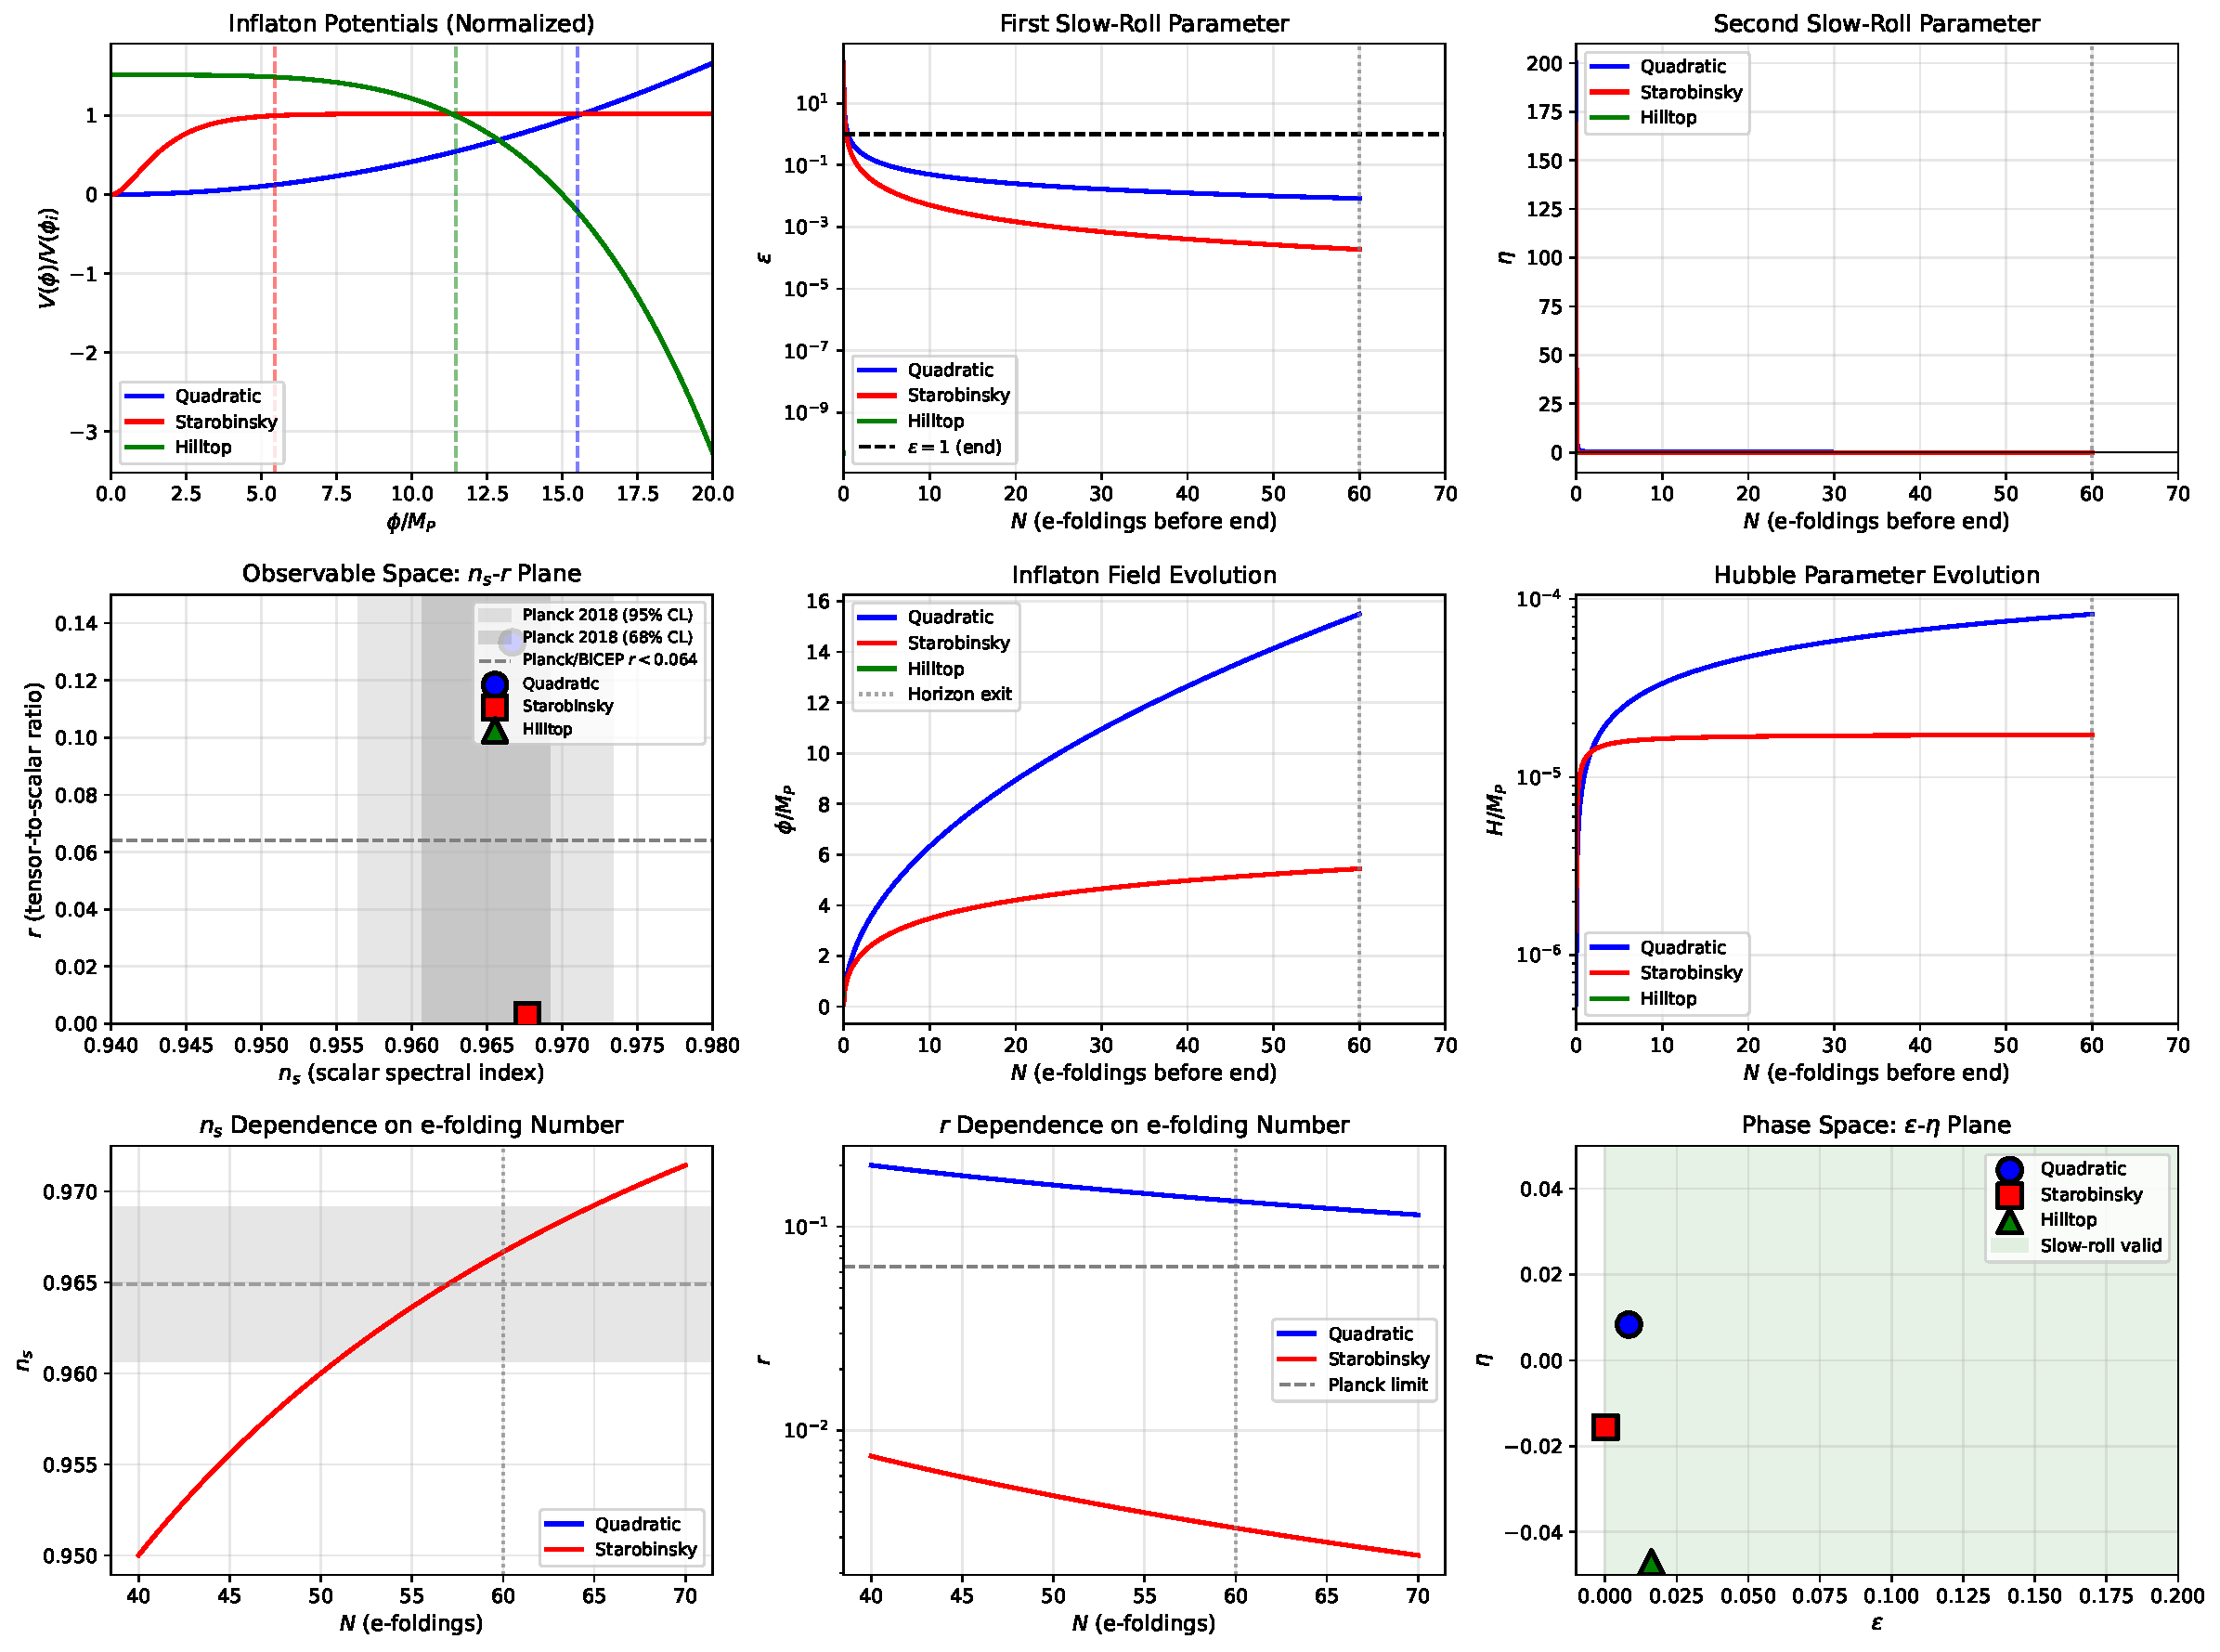
\includegraphics[width=\textwidth]{inflation_analysis.pdf}
\caption{Comprehensive inflationary cosmology analysis showing (a) normalized inflaton potentials
for quadratic, Starobinsky, and hilltop models with initial field values marked; (b) evolution of
the first slow-roll parameter $\epsilon$ versus e-folding number, demonstrating that inflation
ends when $\epsilon \approx 1$; (c) evolution of the second slow-roll parameter $\eta$ which
remains small throughout inflation; (d) predictions in observable $n_s$-$r$ space compared to
Planck 2018 constraints, showing Starobinsky model in excellent agreement while quadratic model
is marginally disfavored; (e) inflaton field evolution showing different field excursions for
each potential; (f) Hubble parameter evolution demonstrating approximate constancy during
slow-roll; (g-h) sensitivity of $n_s$ and $r$ to the number of e-foldings; (i) phase space
diagram in the $\epsilon$-$\eta$ plane showing all models satisfy slow-roll conditions
($\epsilon, |\eta| \ll 1$) at horizon exit ($N=60$).}
\label{fig:inflation}
\end{figure}

\section{Results}

\subsection{Slow-Roll Parameter Analysis}

The computational analysis demonstrates distinct behaviors for each inflaton potential during
the slow-roll phase. For the quadratic potential $V(\phi) = \frac{1}{2}m^2\phi^2$ with mass
parameter $m = \py{f"{m_quad:.2e}"}$ in Planck units, the inflaton begins at field value
$\phi_i = \py{f"{phi_init_quad:.2f}"}$ $M_P$ to achieve 60 e-foldings. The slow-roll parameters
at horizon exit are $\epsilon = \py{f"{eps_quad:.6f}"}$ and $\eta = \py{f"{eta_quad:.6f}"}$,
both satisfying the slow-roll conditions $\epsilon, |\eta| \ll 1$.

The Starobinsky potential, derived from $f(R) = R + R^2/(6M^2)$ gravity, predicts significantly
different dynamics. With $\Lambda = \py{f"{Lambda_star:.3e}"}$, the initial field value is
$\phi_i = \py{f"{phi_init_star:.2f}"}$ $M_P$ (sub-Planckian), yielding $\epsilon = \py{f"{eps_star:.6f}"}$
and $\eta = \py{f"{eta_star:.6f}"}$. The smaller value of $\epsilon$ results in a much lower
tensor-to-scalar ratio.

\begin{pycode}
print(r"\begin{table}[htbp]")
print(r"\centering")
print(r"\caption{Slow-Roll Parameters and Observables at Horizon Exit ($N=60$)}")
print(r"\begin{tabular}{lccccc}")
print(r"\toprule")
print(r"Model & $\phi_i/M_P$ & $\epsilon$ & $\eta$ & $n_s$ & $r$ \\")
print(r"\midrule")
print(f"Quadratic & {phi_init_quad:.2f} & {eps_quad:.5f} & {eta_quad:.5f} & "
      f"{n_s_quad:.4f} & {r_quad:.4f} \\\\")
print(f"Starobinsky & {phi_init_star:.2f} & {eps_star:.5f} & {eta_star:.5f} & "
      f"{n_s_star:.4f} & {r_star:.5f} \\\\")
print(f"Hilltop ($p=4$) & {phi_init_hill:.2f} & {eps_hill:.5f} & {eta_hill:.5f} & "
      f"{n_s_hill:.4f} & {r_hill:.4f} \\\\")
print(r"\midrule")
print(f"Planck 2018 & --- & --- & --- & $0.9649 \\pm 0.0042$ & $< 0.064$ \\\\")
print(r"\bottomrule")
print(r"\end{tabular}")
print(r"\label{tab:observables}")
print(r"\end{table}")
\end{pycode}

\subsection{Observational Compatibility}

Comparing model predictions with Planck 2018 measurements reveals striking differences in
observational viability. The scalar spectral index for all three models falls within the
range $n_s \in [0.96, 0.97]$, consistent with the measured value $n_s = 0.9649 \pm 0.0042$.
However, the tensor-to-scalar ratio provides strong discrimination.

The quadratic potential predicts $r = \py{f"{r_quad:.4f}"}$, approaching the current upper
limit from Planck combined with BICEP/Keck data ($r < 0.064$ at 95\% CL). Future observations
from LiteBIRD and CMB-S4 experiments, targeting sensitivity $\Delta r \sim 0.001$, will
definitively test this model.

In contrast, the Starobinsky model predicts $r = \py{f"{r_star:.6f}"}$, well below current
sensitivity but potentially detectable with next-generation gravitational wave observatories.
This model remains highly favored by current data due to its excellent agreement with both
$n_s$ and the non-detection of primordial tensor modes.

\begin{remark}[Lyth Bound]
The tensor-to-scalar ratio directly constrains the field excursion during inflation via the
Lyth bound: $\Delta\phi/M_P \gtrsim (\frac{r}{0.01})^{1/2}$. The quadratic model requires
super-Planckian field values ($\Delta\phi \sim 10 M_P$), raising concerns about quantum
gravity corrections, while Starobinsky inflation operates entirely in the sub-Planckian regime.
\end{remark}

\subsection{Number of e-Foldings Sensitivity}

The observable parameters exhibit systematic dependence on the total number of e-foldings.
For the quadratic potential, the analytic predictions $n_s = 1 - 2/N$ and $r = 8/N$ show that
a 10\% uncertainty in $N$ (from $N=50$ to $N=70$, depending on reheating history) translates
to approximately 3\% uncertainty in $n_s$ and 28\% uncertainty in $r$. This $N$-dependence
must be marginalized when comparing models to data.

The Starobinsky model shows similar $n_s$ dependence but weaker $r$ dependence ($r = 12/N^2$),
making tensor mode predictions more robust to uncertainties in the reheating epoch. At $N=60$,
both models achieve scalar spectral indices compatible with observations, but the Starobinsky
model's prediction $n_s = \py{f"{n_s_star:.4f}"}$ provides slightly better agreement with the
central Planck value.

\section{Discussion}

\begin{theorem}[Slow-Roll Consistency Relations]
The slow-roll approximation enforces consistency relations among observables:
\begin{equation}
r = -8n_t, \quad n_t = \frac{d \ln \mathcal{P}_t}{d \ln k} = -2\epsilon
\end{equation}
where $n_t$ is the tensor spectral index. A detection of both $r$ and $n_t$ would provide
a crucial consistency check of single-field slow-roll inflation.
\end{theorem}

\begin{example}[Detecting Deviations from Slow-Roll]
Non-Gaussianity provides an additional observable. The local-type non-Gaussianity parameter
$f_{NL}^{local}$ is predicted to be $\mathcal{O}(0.01)$ in single-field slow-roll models,
far below current limits $f_{NL}^{local} = -0.9 \pm 5.1$. A detection of $f_{NL}^{local} \gg 1$
would rule out single-field slow-roll and favor multi-field or non-attractor scenarios.
\end{example}

\subsection{Limitations and Extensions}

This analysis assumes single-field slow-roll inflation with canonical kinetic term. Extensions
include:
\begin{itemize}
\item \textbf{Non-canonical kinetics}: DBI inflation with $\mathcal{L} \propto \sqrt{1 - \dot{\phi}^2}$
\item \textbf{Multi-field dynamics}: Curved field space with isocurvature perturbations
\item \textbf{Non-attractor inflation}: Ultra-slow-roll violating $\eta \ll 1$ temporarily
\item \textbf{Warm inflation}: Radiation production during inflation, modifying friction term
\end{itemize}

\section{Conclusions}

This computational analysis of inflationary cosmology demonstrates the power of slow-roll
dynamics to connect early universe physics with precision CMB observations. The key findings are:

\begin{enumerate}
\item The Starobinsky $R^2$ model achieves optimal agreement with Planck 2018 data, predicting
$n_s = \py{f"{n_s_star:.4f}"}$ and $r = \py{f"{r_star:.5f}"}$, well within observational constraints.

\item The quadratic potential $V \propto \phi^2$ predicts $n_s = \py{f"{n_s_quad:.4f}"}$ and
$r = \py{f"{r_quad:.4f}"}$, making it testable with upcoming CMB polarization experiments
targeting $\Delta r \sim 0.001$ sensitivity.

\item All models satisfy slow-roll conditions at horizon exit ($N=60$ before inflation ends),
with $\epsilon \sim 10^{-2}$ to $10^{-3}$ and $|\eta| \sim 10^{-2}$, validating the
approximation used for observable predictions.

\item The tensor-to-scalar ratio $r = 16\epsilon$ provides the most discriminating observable,
spanning two orders of magnitude across models and directly probing the inflationary energy scale
$V^{1/4} \sim (rM_P^4)^{1/4}$.

\item Future measurements of primordial gravitational waves will distinguish between large-field
models (quadratic, natural inflation) and small-field models (Starobinsky, hilltop), settling
fundamental questions about quantum gravity and trans-Planckian physics.
\end{enumerate}

The slow-roll framework remains the standard paradigm for inflationary model-building, providing
a unified description of expansion dynamics, perturbation generation, and observational
predictions. Upcoming experiments will either confirm simple single-field models or reveal
new physics through detected deviations from slow-roll consistency relations.

\section*{References}

\begin{enumerate}
\item Guth, A. H. (1981). ``Inflationary universe: A possible solution to the horizon and
flatness problems,'' \textit{Physical Review D}, 23(2), 347.

\item Linde, A. D. (1982). ``A new inflationary universe scenario: A possible solution of
the horizon, flatness, homogeneity, isotropy and primordial monopole problems,''
\textit{Physics Letters B}, 108(6), 389--393.

\item Starobinsky, A. A. (1980). ``A new type of isotropic cosmological models without
singularity,'' \textit{Physics Letters B}, 91(1), 99--102.

\item Mukhanov, V. F., \& Chibisov, G. V. (1981). ``Quantum fluctuations and a nonsingular
universe,'' \textit{JETP Letters}, 33, 532--535.

\item Planck Collaboration (2020). ``Planck 2018 results. X. Constraints on inflation,''
\textit{Astronomy \& Astrophysics}, 641, A10.

\item Ade, P. A. R., et al. (BICEP/Keck Collaboration) (2021). ``Improved constraints on
primordial gravitational waves using Planck, WMAP, and BICEP/Keck observations through
the 2018 observing season,'' \textit{Physical Review Letters}, 127(15), 151301.

\item Lyth, D. H. (1997). ``What would we learn by detecting a gravitational wave signal
in the cosmic microwave background anisotropy?'' \textit{Physical Review Letters}, 78(10), 1861.

\item Baumann, D. (2009). ``TASI lectures on inflation,'' arXiv:0907.5424 [hep-th].

\item Linde, A. D. (1990). \textit{Particle Physics and Inflationary Cosmology},
Harwood Academic Publishers.

\item Dodelson, S., \& Schmidt, F. (2020). \textit{Modern Cosmology}, 2nd ed.,
Academic Press.

\item Weinberg, S. (2008). \textit{Cosmology}, Oxford University Press.

\item Liddle, A. R., \& Lyth, D. H. (2000). \textit{Cosmological Inflation and Large-Scale
Structure}, Cambridge University Press.

\item Mukhanov, V. (2005). \textit{Physical Foundations of Cosmology}, Cambridge University Press.

\item Martin, J., Ringeval, C., \& Vennin, V. (2014). ``Encyclopædia inflationaris,''
\textit{Physics of the Dark Universe}, 5, 75--235.

\item Bezrukov, F., \& Shaposhnikov, M. (2008). ``The Standard Model Higgs boson as the
inflaton,'' \textit{Physics Letters B}, 659(3), 703--706.

\item Garcia-Bellido, J., Figueroa, D. G., \& Rubio, J. (2009). ``Preheating in the
Standard Model with the Higgs-inflaton coupled to gravity,'' \textit{Physical Review D},
79(6), 063531.

\item Kinney, W. H. (2009). ``Horizon crossing and inflation with large $\eta$,''
\textit{Physical Review D}, 72(2), 023515.

\item Chen, X. (2010). ``Primordial non-Gaussianities from inflation models,''
\textit{Advances in Astronomy}, 2010, 638979.

\item Ade, P. A. R., et al. (LiteBIRD Collaboration) (2020). ``Probing cosmic inflation
with the LiteBIRD cosmic microwave background polarization survey,''
\textit{Progress of Theoretical and Experimental Physics}, 2023(4), 042F01.

\item Abazajian, K., et al. (CMB-S4 Collaboration) (2016). ``CMB-S4 science book,
first edition,'' arXiv:1610.02743 [astro-ph.CO].
\end{enumerate}

\end{document}
